\documentclass{beamer}
\renewcommand\textbullet{\ensuremath{\bullet}}

\usepackage{opencg3-spec}
\usepackage{opencg3-spec-beamer}
\usepackage{xspace,bookmark,lmodern,mathtools,color,multido,ulem,upquote,tabularx}
\usepackage[T1]{fontenc}
\usefonttheme[onlymath]{serif}

\newcommand{\Version}[0]{Version 0.2.2}
\newcommand{\PrjName}{OpenCG\texorpdfstring{\textsuperscript{3}}}
\newcommand{\PrjNameFull}{Open Command-oriented\\Geometric Graphics Generator}
\newcommand{\PrjSpec}{\PrjName{} Spec \Version}

\title[\PrjSpec]{\PrjNameFull}
\subtitle{\small \PrjSpec}


\author[KVD \and ADL]{Dong Nai-Jia \inst{1} \and Lin Yong-Siang \inst{2}}
\institute{	\inst{1} National Chiao Tung University\\Department of Computer Science \and
			\inst{2} National Taiwan University\\Department of Agricultural Chemistry}
\date[\today]{\today}


\begin{document}


\begin{frame}
	\titlepage
\end{frame}


\section{Overview}

\subsection{Illustration}

\begin{frame} \frametitle{Perspective Projection}

	\begin{figure}[t]
		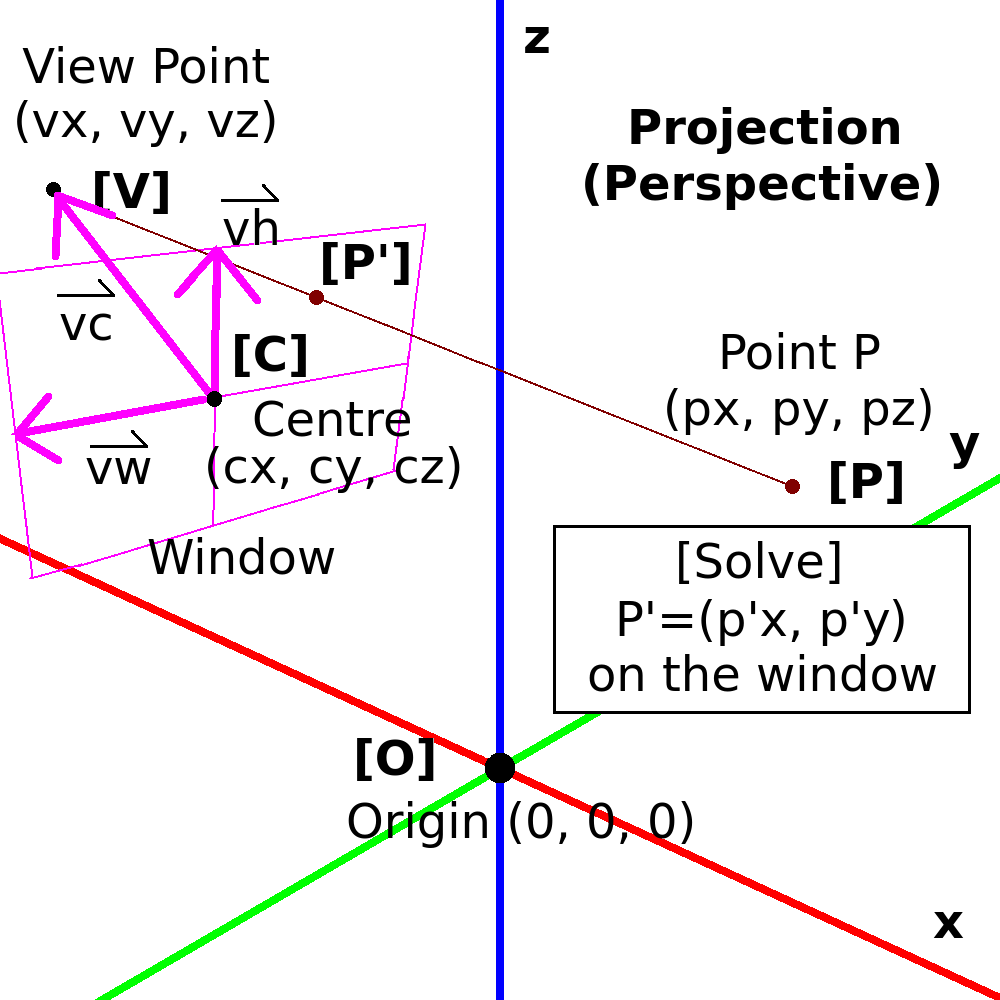
\includegraphics[width=.5\columnwidth]{fig/perspective-projection.png}
		\caption{Projection in Euclidean $\mathbb{R}^3$ Space}
	\end{figure}

\end{frame}

\subsection{Definitions}

\begin{frame}[t] \frametitle{Command Tokens}

	\begin{block}{Regular Expressions}
		$\MSN \coloneqq \{\ \alpha \mid \alpha \in \texttt{[0-9]+} \ \}$ \\ [.24em]
		$\MSR \coloneqq \{\ \alpha \mid \alpha \in \texttt{[+\textbackslash-]?([0-9]*[.])?[0-9]+}\ \}$ \hfill
		$\Rightarrow \MSR \supset \MSN \ $ \\ [.24em]
		$\MSS \coloneqq \{\ \alpha \mid \alpha \in \texttt{\SingleQuote(.*?)\SingleQuote|[.0-9A-Za-z+\textbackslash-]+} \ \}$ \hfill
		$\Rightarrow \MSS \supset \MSR \ $ \\ [.24em]
		$\MSW \coloneqq \{\ \alpha \mid \alpha \in \texttt{[ \textbackslash{}t]} \}$ \hfill whitespace
	\end{block}

	\begin{block}{Descriptions}
		\begin{itemize}
			\item The matching mechanism abides by the maximal munch rule.
			\item Each command is whitespace-insensitive except being quoted by a pair of single quotation marks (\SingleQuote).
		\end{itemize}
	\end{block}

\end{frame}

\begin{frame}[t] \frametitle{Command Grammars}

	\begin{block}{Context-Free Expansions}
		$\left.\CMD \EXP \ARG \CMD \SEP \,\text{;}\, \SEP \,\texttt{EOL} \right.$ \\ [.24em]
		$\left.\ARG \EXP \TUP(\ARG) \SEP \VCT(\ARG) \SEP \SET(\ARG) \SEP
		 \LST(\ARG) \SEP \LST(\ARG, \ARG, \cdots, \ARG) \SEP \MSN \SEP \MSR \SEP \MSS \right.$ \\ [.27em]
		$\left.\text{%
		\begin{tabular}{@{}l}%
			$\TUP(\Pi) \EQV \Tup{\Pi}{n} \EXP \texttt{\TupBrkL}     \ \, \Sigma(\Pi, n) \ \, \texttt{\TupBrkR}$ \\ [.24em]
			$\VCT(\Pi) \EQV \Vct{\Pi}{n} \EXP \texttt{\VctBrkTextL} \ \, \Sigma(\Pi, n) \ \, \texttt{\VctBrkTextR}$ \\ [.24em]
			$\SET(\Pi) \EQV \Set{\Pi}{n} \EXP \texttt{\SetBrkL}     \ \, \Sigma(\Pi, n) \ \, \texttt{\SetBrkR}$
		\end{tabular}} \right\|$%
		\begin{tabular}{@{}l}%
			$\ \Sigma(\Pi, n) \EXP \underbrace{\Pi \ \cdots \ \Pi}_{n \ \text{items}} \quad\,\ \text{(identical)}$ \\ [1.725em]
			$\ \LST(\Pi) \EQV \Lst{\Pi}{n} \EXP \texttt{\LstBrkL} \ \, \Sigma(\Pi, n) \ \, \texttt{\LstBrkR}$
		\end{tabular} \\ [.24em]
		$\left.\LST(\Pi_1,\Pi_2,\cdots,\Pi_{n-1},\Pi_n) \EQV \kern.05em \LstFull{\Pi_1\,\Pi_2\cdots\Pi_{n-1}\,\Pi_n} \EXP
		 \texttt{\LstBrkL} \ \, \Pi_1\cdots\Pi_n \ \, \texttt{\LstBrkR}\right.$
	\end{block}

	\begin{block}{Descriptions}
		\begin{itemize}
			\item Each command starts from $\CMD$ and ends with a \texttt{;} or an \texttt{EOL}.
			\item Non-terminal symbol expansions are prior than function expansions except that it is used in the form of describing types of a command.
		\end{itemize}
	\end{block}

\end{frame}


\section{Commands}

\subsection{Window}

\begin{frame}[t] \frametitle{Create a Window}

	\begin{block}{Command} \newcolumntype{R}{>{\raggedleft\arraybackslash}X}
		\begin{tabularx}{\textwidth}{@{}l@{}l@{}l@{}l@{}R}
			\InstrName{create window} &
				\ParamMust{\StrName{label}} &
				\ParamMust{\TupName{\MSR}{3}{coord}} &
				\ParamMust{\TupName{\Vct{\MSR}{3}}{3}{dirct}} & \InstrItem
		\end{tabularx}
	\end{block}

	\begin{block}{Parametres} \begin{itemize}
		\ParamItem{label} the unique name of the window
		\ParamItem{coord} the coordinate $(c_x, c_y, c_z)$ of the window centre
		\ParamItem{dirct} the width $\vec{v_w}$, height $\vec{v_h}$, and the view point $\vec{v_c}$
	\end{itemize} \end{block}

	\begin{block}{Examples}
		\CommandEx{create window main \TupText{0 0 1} \TupText{\VctText{1 0 0} \VctText{0 1 0} \VctText{0 0 1}}}
	\end{block}

\end{frame}

\begin{frame}[t] \frametitle{Delete a Window}

	\begin{block}{Command} \newcolumntype{R}{>{\raggedleft\arraybackslash}X}
		\begin{tabularx}{\textwidth}{@{}l@{}l@{}R}
			\InstrName{delete window} &
			  	\ParamOptl{\StrName{message}} & \InstrItem
		\end{tabularx}
	\end{block}

	\begin{block}{Parametres} \begin{itemize}
		\ParamItem{message} the text string printed right after exit
	\end{itemize} \end{block}

	\begin{block}{Examples}
		\CommandEx{delete window}
		\CommandEx{delete window \SingleQuote Have a nice day.\SingleQuote}
	\end{block}

\end{frame}

\subsection{Points}

\begin{frame}[t] \frametitle{Create Points}

	\begin{block}{Command} \newcolumntype{R}{>{\raggedleft\arraybackslash}X}
		\begin{tabularx}{\textwidth}{@{}l@{}l@{}l@{}R}
			\InstrName{create point } &
			  	\ParamMust{\SetOptl{\StrName{label}}{}} &
			  	\ParamMust{\TupName{\MSR}{3}{coord}} & \InstrItem \\
			\InstrName{create point } &
				\ParamMust{\Tup{\StrName{label}}{n}} &
				\ParamMust{\Tup{\TupName{\MSR}{3}{coord}}{n}} & \InstrItem
		\end{tabularx}
	\end{block}

	\begin{block}{Parametres} \begin{itemize}
		\ParamItem{label} the name of the point
		\ParamItem{coord} the coordinate $(p_x, p_y, p_z)$ of the point
	\end{itemize} \end{block}

	\begin{block}{Examples}
		\CommandEx{create point \SingleQuote origin\SingleQuote \ \ \ \TupText{0 0 0}}
		\CommandEx{create point \SetText{X-1 X-2} \ \TupText{1 0 0}}
		\CommandEx{create point \TupText{Y-1 Z-1} \TupText{\TupText{0 1 0}\TupText{0 0 1}}}
	\end{block}

\end{frame}

\begin{frame}[t] \frametitle{Delete Points}

	\begin{block}{Command} \newcolumntype{R}{>{\raggedleft\arraybackslash}X}
		\begin{tabularx}{\textwidth}{@{}l@{}l@{}R}
			\InstrName{delete point } &
				\ParamMust{\SetOptl{\StrName{label}}{}} & \InstrItem
		\end{tabularx}
	\end{block}

	\begin{block}{Parametres} \begin{itemize}
		\ParamItem{label} the name of the point
	\end{itemize} \end{block}

	\begin{block}{Examples}
		\CommandEx{delete point \ origin}
		\CommandEx{delete point \SetText{origin \SingleQuote random-point\SingleQuote}}
	\end{block}

\end{frame}

\subsection{Attribute}

\begin{frame}[t] \frametitle{Create Attributes}

	\begin{block}{Command} \newcolumntype{R}{>{\raggedleft\arraybackslash}X}
		\begin{tabularx}{\textwidth}{@{}l@{}l@{}l@{}R}
			\InstrName{create attrib} &
				\ParamMust{\SetOptl{\StrName{label}}{}} &
				\ParamMust{\LstFull{\StrName{type} \ \StrName{key} \ \ArgName{value}}} & \InstrItem \\
			\InstrName{create attrib} &
				\ParamMust{\Tup{\StrName{label}}{n}} &
				\ParamMust{\Lst{\LstFull{\StrName{type} \ \StrName{key} \ \ArgName{value}}}{n}} & \InstrItem
		\end{tabularx}
	\end{block}

	\begin{block}{Parametres} \begin{itemize}
		\ParamItem{type} the type of the object
		\ParamItem{key} the property of the object
		\ParamItem{value} the value of the property
	\end{itemize} \end{block}

	\begin{block}{Examples}
		\CommandEx{create attrib \SetText{surface} \LstText{surface translucency 0.85}}
		\CommandEx{create attrib \TupText{magenta auxiliary} \EOLText
								 \LstText{\LstText{point fill-hsv \TupText{300 1.0 1.0}} \LstText{line style dashed}}}
	\end{block}

\end{frame}

\subsection{Miscellaneous}

\begin{frame}[t] \frametitle{Assign an Operation}

	\begin{block}{Command} \newcolumntype{R}{>{\raggedleft\arraybackslash}X}
		\begin{tabularx}{\textwidth}{@{}l@{}l@{}l@{}l@{}R}
			\InstrName{assign opratn} &
				\ParamMust{\StrName{action}} &
				\ParamMust{\StrName{type}} &
				\ParamOptl{\MSNName{repeat}\ \ValueDefn{=\infty}} & \InstrItem
		\end{tabularx}
	\end{block}

	\begin{block}{Parametres} \begin{itemize}
		\ParamItem{action} the name of the action
		\ParamItem{type} the type of the object applying the action
		\ParamItem{repeat} the amount of the commands emitting operations
	\end{itemize} \end{block}

	\begin{block}{Examples}
		\CommandEx{assign opratn create point 2}
		\CommandEx{x-axis \TupText{1 0 0}; y-axis \TupText{0 1 0}}
		\CommandEx{// Back To Normal}
	\end{block}

\end{frame}


\section{}

\begin{frame}
	\begin{center}
		\TmpGray{This page is intentionally left blank.}
	\end{center}
\end{frame}


\end{document}

